%!TeX root = ../main.tex
\section*{Guest Lecture 2a, 13/03/2018}
These lectures, by Ori Ganor, will discuss Chern-Simons theory.
This is a $3$-dimensional gauge theory of a Lie-algebra valued $1$-form $A$, with action
\begin{align*}
S &= \frac{k}{4 \pi} \int \tr \left( A \wedge dA + \frac{2}{3} A \wedge A \wedge A\right)\\
&= \frac{k}{4 \pi} \int \varepsilon^{\mu \nu \sigma} \left[A_{\mu a} \partial_\nu A_\sigma^a + \frac{2}{3} f_{abc} A_\mu^a A_\nu^b A_\sigma^c \right] d^3x.
\end{align*}
The explicit appearance of $\varepsilon$ means that this theory is not invariant under \me{one of (?)} $P$ or $T$.
Today we just focus on the Abelian case, where the second term vanishes.

We can consider an action of the form
\[
S_{\text{TOT}} = S_{\text{YM}} + S_{\text{CS}} = \frac{1}{4g^2} \int \tr F \wedge F + S_{\text{CS}}.
\]
Recall some (semiclassical because there might be quantum anomalies) dimensional analysis.
In 4D $g^2$ is dimensionless (except really not because it depends on the energy scale via dimensional regularization) while in 3D it has dimensions of mass.
There are two ways to remember this: one is that
\[
D_{\mu} = \partial_\mu + i A_\mu
\]
so that $A_\mu$ has dimensions of mass, and look at the action $(4g^2)^{-1} \int F^2 \,d^3x$.
\me{There was also a mention of the Ahoromov-Bohm phase $e^{i q \oint A_\mu d^\mu x}$.}

In the low energy limit, $g^2 \to \infty$, so we can forget about the YM terms in the action, so the CS term dominates the IR physics.
Furtheromre, the first term in the CS action is more important.

\subsection*{Quantum Hall Effect}
There is both an integer effect (understood) and a fractional one (an open problem.)
We see how Chern-Simons applies to them.

Classically, the setup is as follows.
We have a 2D thin-film sample in a STRONG (order of teslas) magnetic field, with a voltage $V_y$ in the $y$ direction and a current $I_x$ in the $x$ direction.
The resistivity is $\rho_H = V_y/I_x$.
If the charge carriers have charge $q$, density $n$, and velocity $v_x$, then
\[
\frac{V_y}{I_x} = \frac{E_y L}{J_x L} = \frac{E_y}{J_x}
\]
Since the current density is $J_x = nq v_x$,
\[
\rho_H = \frac{E_y}{n q v_x} = \frac{B}{nq}
\]
as things balance out with the magnetic force.
More generally there is a resistivity \emph{matrix} $\rho_{ij}$ with $\rho_{ij} J_j = E_i$, and we can ask what the values of $\rho_{ij}$ are.

This is a plot of $\rho_{xy}$ in units of $h/e^2$:
\begin{center}
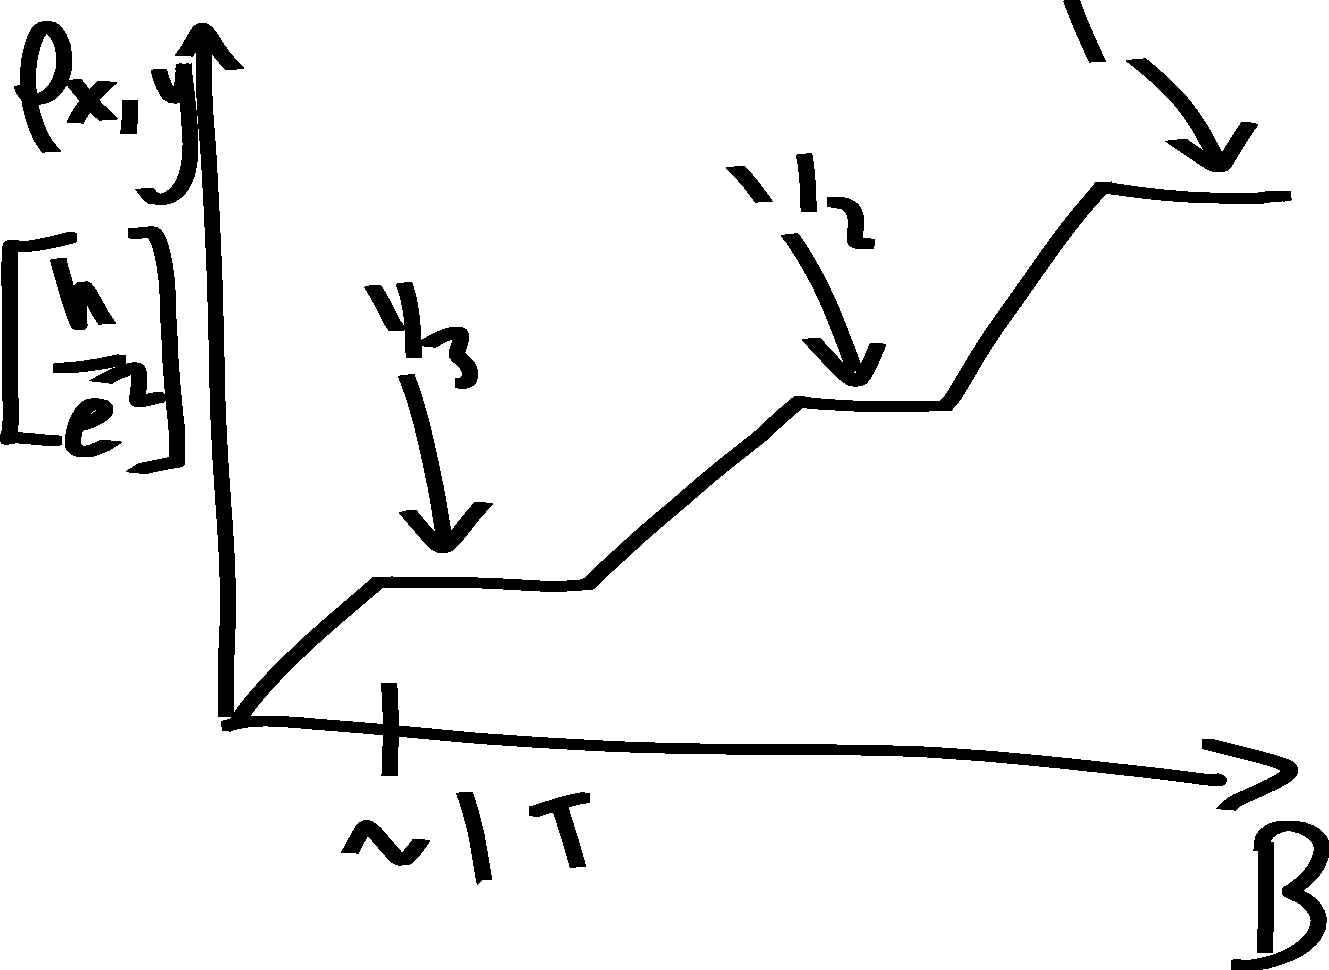
\includegraphics[width = 5in]{fig/quantum-hall-graph.pdf}
\end{center}
$\rho_{xx}$ on the other hand is roughly the same valueof $\rho_{xy}$, but it falls to zero at the plateaus.
This reflects an ``incompressible quantum state.''

This can be explained as follows: \me{(but note that I missed some parts of the following)} Suppose there's a single particle of charge $q$.
We get gapped states each with large degeneracy, via $\hbar \omega_B = q B/m$.
In particular, each particle takes fundamental flux $\phi_0 = 2 \pi \hbar / |e|$, so the total number of states at each energy is
\[
\frac{BA}{\phi_0}
\]
where $A$ is the area of the sample.
Idea is that each state has a ``bubble'' of flux around it and these don't overlap.
The plateaus happend because disorder/impurities spread out the degneracies.
The edges of these spreads are localized nonconductive states, so the first and last part of the increase in $B$ doesn't create any more conductivity.

The \emph{fractional} effect is more mysterious and more difficult to get.
It happens for fractions of the form $n/(2mn \pm 1)$.
It's mostly open why it happens.
One reason is that it depends heavily on the electron-electron interactions.
There are lots of these: if $\nu = 1/3$ then there are something like $\binom{N}{N/3}$ states, which is a \emph{lot.}

\subsection*{Connection to field theory}
Let $A = A_{\text{ext}}$ be the background EM field, with $\mathbf B = B \hat z$ and $\mathbf E = V_y \hat y$.
We write $\psi$ for the electrons in the sample.
Consider a partition function of the form
\[
\int e^{-\frac{i}{\hbar} S[A, \psi)]}.
\]
Here the effective action is
\[
S = \frac{k}{4 \pi} \int A \wedge dA
\]
This is topological, so how does it come from a condensed matter system?
It's reasonable if there are no propagating degrees of freedom.

We have
\[
\left \langle J_i(X) \right \rangle_A = \left \langle \frac{\delta S}{\delta A(x)} \right \rangle = \int \left( \frac{\delta S}{\delta A} e^{\frac{i}{\hbar} S}\right) \mathcal D \psi = \frac{\hbar}{i} \frac{\delta}{\delta A} \int e^{\frac{i}{\hbar} S} \mathcal D \psi = \frac{\delta}{\delta A} \left( e^{\frac{iS}{\hbar}} \right)
\]
so that
\[
\left \langle J_i \right \rangle =\frac{\delta S}{\delta A} = \frac{k}{2 \pi} \varepsilon_{ijk} F_{jk}
\]
Macroscopically, $J_i = k \varepsilon_{ij} E_j /2 \pi$, so $\sigma_{xy} = k/2 \pi$ and $\rho_{xy} = 2 \pi /k$ (where $\hbar = e = 1$.)

We now put the theory on a $2$-torus, so that
\[
S = \frac{k}{4 \pi} \int A \wedge dA = \frac{k}{4 \pi} \int (A_2 A_1 - A_1 A_2) \intd t \intd x \intd y = \frac{k}{2 \pi} \int A_2 \dot A_1 + \text{boundary terms} \intd t \intd x \intd y
\]\
and impose the gauge $A_0 = 0$.

There is one problem here: we still have a equation from varying $A_0$ that we'd now leave out, so we include it manually:
\[
0 = \frac{\delta S}{\delta A_0} = F_{12}.
\]
This means there's no field strength!

Furthermore, there are topological obstructions that can't be gauged away, namely the winding numbers
\[
\frac{1}{2 \pi} \oint_{C_i} A_i \intd x^i
\]
where $C_1, C_2$ are noncontractable loops around the torus.

\section*{Guest Lecture 2b, 15/03/2018}
Recall from last time we discussed the relationship between the quantum Hall effect and an (effective) Chern-Simons field theory.
\me{There was a more detailed recap that I won't repeat.}
There is one problem with this theory: there's a coupling $A_\mu J^\mu$ for some current $J^\mu$, so you get terms like $\int \langle J^\mu j^\nu \rangle A_\mu A_\nu \intd^3 x$ that are nonlocal.
However, this turns out not to be a problem: there is an \emph{energy gap} (called a \emph{mass gap} in field/high-energy theory) and this will make the nonlocal correlators fall off exponentially, so that (at least in the IR limit) the nonlocal correlators wind up being $\delta$ functions.

In order to explain the integer quantum Hall effect we will want the parameter $k$ to be an integer, as it's related to the filling fraction $\nu$.
We now explain why.

Consider Chern-Simons theory on a torus $T^2$, with $1$-periodic \me{(actually I think it should be $2 \pi$-periodic)} coordinates $x_1, x_2$.
Write $A = a_1 \intd x_1 + a_2 \intd x_2$.
We can set $A_0 = 0$ by gauge invariance, which then requires imposing $F_{12} = 0$, so there is no field strength, and
\begin{align*}
S = \frac{k}{4 \pi} \int (a_2 \dot a_1 - a_1 \dot a_2) \intd t = \frac{k}{2 \pi} \int a_2 \dot a_1 \intd t,
\end{align*}
which is a $(0+1)$-dimensional theory, i.e.~regular old quantum mechanics.

In particular, we should have canonical commutation relations
\[
[a_2, a_1] = - \frac{2 \pi i}{k}.
\]
We also need to determine the Hilbert space.
Recall that there is a ``residual'' gauge transformation $\Lambda = 2 \pi N \intd x$ for $N \in \mathbb Z$.
It isn't single-valued, but $e^{i \Lambda} \in \grp U(1)$ is, and under this transformation
\begin{align*}
A &\mapsto a_1 \intd x_1 + a_2 \intd x_2 + 2 \pi N \intd x_1\\
a_1 &\mapsto A_1 + 2 \pi N
\end{align*}
and similarly for $a_2$.
In particular, we get $a_1 \sim a_1 + 2 \pi$, $a_2 \sim a_2 + 2 \pi$, so that \emph{momentum} is periodic.
Therefore to make things single-valued we should look instead at \emph{Wilson loops} $W_j = e^{i a_j} = e^{i \oint_{c_j} A}$, which are just holonomies of the connection.

The commutator is now
\[
W_1 W_2 W_1^{-1} W_2^{-1} = e^{-[a_1,a_2]} = e^{-2 \pi i /k} =: \omega.
\]
In particular, $W_2^{-1} W_1 W_2 = \omega^{-1} W_1$.
\me{I'm not sure whether $W$ or $w$ was intended, but I'm choosing the former to distinguish it better from $\omega$.}

The $W_i$ are unitary operators, so we can ask what their matrix representations are.
Notice that if $\lambda$ is an eigenvalue of $W_i$, then the commutation relation implies that so is $\omega \lambda$.
We can (up to a phase that we won't write) therefore write the operators as
\[ W_1 = 
\begin{bmatrix}
1 & 0 &0 & \dots & 0\\
0 & \omega & 0 & \dots & 0\\
0 & 0 & \omega^2 & \dots & 0\\
\vdots & \vdots & \vdots & \ddots\\
0 & 0 & 0 &  & \omega^{n-1}
\end{bmatrix}, \quad
W_2 =
\begin{bmatrix}
0 & 1 & 0 & \dots\\
0 & 0 & 1 & \dots\\
\vdots & \vdots & \vdots & \ddots
\end{bmatrix}.
\]
This only works with finite dimensions if $k$ is an integer.

\subsection*{Geometric quantization}
Define $u = a_1 + ia_2$, $\bar u = a_1 -ia_2$.
Then
\[
[u,\bar u] = \frac{4 \pi}{k}
\]
so we have
\[
u^\dagger = \bar u = \frac{4 \pi}{k} \partial_u
\]
Thus the wavefunctions won't be general functions of $a_1, a_2$, but \emph{holomorphic} functions of $u$.

There is a further problem: the obvious inner product $\braket{\chi}{\psi} \defeq \int \chi^*(u) \psi(u) \intd^2u$ won't work:
\begin{align*}
\braket{\chi}{\frac{d}{du} \psi} &= \int \chi^* \frac{d \psi}{d u} \intd^2 u\\
&= - \int \frac{d \chi^*}{d u} \psi \intd^2u\\
&= 0
\end{align*}
since $\chi^*$ is antiholomorphic.
To fix this, we can instead define the inner product by
\[
\braket{\chi}{\psi} = \int \chi^*(u) \psi(u) e^{- \frac{k}{4 \pi}|u|^2}\intd^2u
\]
so that
\begin{align*}
\braket{\chi}{\frac{d}{du} \psi} &= \int \chi^* \frac{d \psi}{du} e^{-\frac{k}{4 \pi}|u|^2} \intd^2u\\
&= - \int \frac{d \chi^*}{du} \psi \intd^2u + \frac{k}{4 \pi} \int \bar u \chi^* \psi e^{-\frac{k}{4 \pi} |u|^2} \intd^2 u,
\end{align*}
which works out.

Another issue: To make things well-defined on $T^2$ we need
\begin{align*}
\chi^*(u) \psi(u) e^{-\frac{k}{4 \pi}|u|^2} = \chi^*(u+ 2 \pi) \psi(u+ 2 \pi) e^{-\frac{k}{4 \pi}|u+ 2 \pi|^2} = \chi^*(u + 2 \pi i) \psi(u + 2 \pi i) e^{-\frac{k}{4 \pi}|u + 2 \pi i|^2},
\end{align*}
which we can get by requiring
\begin{align*}
\psi(u + 2 \pi) &= \psi(u) e^{\frac{k}{2 \pi} (u+ \pi)}\\
\psi(u + 2 \pi i) &= \psi(u) e^{\frac{k}{2 \pi} (-iu+ \pi)}.
\end{align*}

What do holomorphic functions satisfying the above look like?
If $k \not \in \mathbb Z$ there are none, while if it is there are $k$ linearly independent solutions
\[
\psi_j(u) = e^{\frac{k}{8 \pi} u^2} \sum_{n = - \infty}^\infty q^{\frac{(kn+j)^2}{2k}} e^{i(kn+j)u}
\]
where $q = e^{-2 \pi}$.
These are \emph{theta functions.}

\subsection*{Higher dimensions}
We now want to quantize some compact, $2M$-dimensional symplectic phase space with form $\omega$.
If we have local coordinates, we can quantize things like $[x^l, x^j] = - i \omega^{lj}$, but this is hard \me{or impossible (?)}.
On the other hand, if we have a complex structure and resulting complex coordinates $z^\alpha, \bar z^{\bar \alpha}$ such that
$\omega_{\alpha \bar \beta} = - \omega_{\bar \beta \alpha}$ and $\omega_{\alpha \beta} = \omega_{\bar \alpha \bar \beta} = 0$, then we can locally write $\omega_{\alpha \bar \beta} = \partial_\alpha \partial_{\bar \beta} K$ for a \emph{K\"ahler function} $K$, and this will give
\[
[\partial_{\bar \alpha} K , z^{\bar l}] = \delta_{\bar \alpha}^{\bar l}
\]
In our previous example, we had $K = k |u|^2 /4 \pi$ and $\omega = k \intd u \wedge d \bar u /4 \pi$.

Note that the K\"ahler function isn't actually globally defined, but changes in different coordinate patches; it's a section of a complex line bundle.
More generally, it doesn't actually need to be a K\"ahler structure, we just need a choice of complex line bundle (the ``prequantum line bundle.'')

\subsection*{Fractional Quantum Hall Effect}
What happens when our sample has a boundary?
Under the transformation $A \mapsto A+ d \Lambda$, 
\[
\frac{k}{4 \pi} \int_M A \wedge dA \mapsto \frac{k}{4 \pi} \int_M A \wedge dA + \frac{k}{4 \pi} \int_{\partial M} \Lambda dA
\]
so the action isn't gauge-invariant.

To fix this we add boundary states that aren't gauge invariant either; we can think of them as left-moving fermions.
In this case, when we wrap $\theta$ around one time, we create another state that cancels out the problematic term in the action.
\me{I think: I didn't really follow this discussion.}

In particular, this seems to require things to be integral.
That's why the fractional effect is so surprising!

One partial explanation: There is a coupling $J \wedge A$ with $d*J = 0$.
If $*J = da$, then the can think of it as its own Chern-Simons term
\[
\frac{\tilde k}{4 \pi} \int a \wedge da
\]
so that
\[
S = \int da \wedge A + \frac{k}{4 \pi} a \wedge da
\]
\me{Not sure if the coefficients are right here.}
Naively integrating out $a$ then gives an effective Chern-Simons action with \emph{fractional} $k$
This translates to the statement that
\[
*J = - \frac{1}{2 \pi \tilde k} * dA.
\]

\subsection*{Nonabelian Chern-Simons}
Recall that the general action is
\[
S = \frac{k}{4 \pi} \int \tr\left(A \wedge dA + \frac{2}{3} A \wedge A \wedge A \right).
\]
If you quantize in $A_0 = 0$, then $F = 0$.
The Hilbert space of states on a Riemann surface will be solutions of $0 = dA + A \wedge A$, so it's the moduli space of flat connections.
This space has a symplectic form and you can geometrically quantize.
The resulting Hilbert space has to do with Jones polynomials, which you can view in this context as the holonomy around knots/links.
(These are the only interesting operators because the local ones all vanish.)

In answer to a question asked after lecture: There is one big, nonobvious leap in Witten's paper on this, which has to do with the passage from Chern-Simons to CFT in the nonabelian case.
Then the wavefunctions $\psi$ aren't just ordinary functions (actually, even in the original case they depended on a choice of complex structure) but have to do with characters of the affine Lie algebra of the group $G$.